\documentclass{article}

\usepackage[preprint]{tmlr}

\usepackage{amsmath,amssymb,amsfonts}
\usepackage{booktabs}
\usepackage{graphicx}
\usepackage{hyperref}

\renewcommand{\arraystretch}{1.3}
\setlength{\abovetopsep}{6pt}

\title{Grassmannian Geodesic Distance Detects Batch Structure in Metabolomics\\but Does Not Predict Cross-Cohort Classifier Degradation}

\author{\name Elliot Tower \\
      \email elliot@elliottower.ai}

\begin{document}
\maketitle

\begin{abstract}
We test whether the geodesic distance between cohort-specific PCA subspaces on the Grassmannian predicts cross-cohort classifier failure in metabolomics. Using 1{,}039 serum samples from the MTBLS7260 pancreatic cancer study (15 analytical plates, LC-MS HILIC biogenic amines), we compute top-$k$ PCA subspaces per plate and measure pairwise geodesic distances on $\mathrm{Gr}(10, 1022)$. Plate subspaces are well-separated from a permutation null ($z = 31.56$, $p < 0.001$, 1{,}000 permutations), confirming that batch structure is geometrically detectable. Geodesic distance does not predict the pairwise AUC gap between internal and external validation (Spearman $\rho = 0.040$, $p = 0.684$, 105 plate pairs); a random forest robustness check yields a marginally stronger but still non-significant correlation ($\rho = 0.180$, $p = 0.066$). Three na\"{i}ve baselines (centroid distance, domain-classifier AUC, variance ratio) perform comparably, with no score exceeding $|\rho| = 0.19$. Per-plate sample sizes ($\sim$72) produce AUC estimates too noisy for any geometric or distributional signal to resolve. Grassmannian geometry detects batch-driven subspace divergence---a necessary condition for transportability failure---but predicting classifier degradation requires cohorts large enough for stable performance estimates.
\end{abstract}

\section{Introduction}

Clinical metabolomics studies routinely report high internal classification accuracy, then fail to reproduce when applied to independent cohorts acquired on different instruments, in different laboratories, or at different times \citep{broadhurst2006statistical}. The transportability gap---the difference between internal cross-validation AUC and external validation AUC---reflects systematic differences in the data-generating process across cohorts: instrument drift, batch effects, population differences, and sample handling variation \citep{wehrens2016improved}.

Standard practice addresses this gap by applying batch correction algorithms \citep{johnson2007adjusting} or reporting external validation directly. These approaches do not characterize \emph{how much} the cohort-specific data manifolds diverge. A geometric measure of cross-cohort subspace distance that predicted classifier degradation would enable prospective flagging of transportability risk before any classifier is trained.

We test this idea directly. Given $C$ independent cohorts with a shared feature space, we extract the top-$k$ PCA subspace from each and measure pairwise geodesic distances on the Grassmannian manifold $\mathrm{Gr}(k, d)$. The geodesic distance between two $k$-dimensional subspaces is the $\ell_2$ norm of their principal angles \citep{bjorck1973numerical, ye2016schubert}:
\begin{equation}
d_{\mathrm{Gr}}(V_1, V_2) = \left(\sum_{i=1}^{k} \theta_i^2\right)^{1/2}
\end{equation}
where $\theta_1, \ldots, \theta_k$ are the principal angles between $V_1$ and $V_2$, computed as the singular values of $U_1^\top U_2$ for orthonormal bases $U_1, U_2$. Principal angles of zero indicate shared directions; $\pi/2$ indicates orthogonal directions.

\paragraph{Contributions.}
\begin{itemize}
\item \textbf{Geometric batch detection (\S\ref{sec:batch}).} Grassmannian geodesic distance between plate subspaces achieves $z = 31.56$ against a plate-label permutation null---plates occupy geometrically distinct subspaces.
\item \textbf{Prediction null result (\S\ref{sec:prediction}).} Geodesic distance does not predict the pairwise AUC gap (logistic regression: $\rho = 0.040$, $p = 0.684$; random forest: $\rho = 0.180$, $p = 0.066$). Three na\"{i}ve baselines perform comparably, with the best achieving $|\rho| = 0.188$.
\item \textbf{Scope (\S\ref{sec:discussion}).} The geometric test detects batch structure---a necessary condition for classifier degradation---but per-plate sample sizes ($\sim$72) are too small for the prediction test to resolve any signal.
\end{itemize}


\section{Data}

We use MetaboLights accession \textbf{MTBLS7260} \citep{leonletelier2024contributions}, a pancreatic cancer study from the PLCO screening trial. The dataset contains 1{,}039 serum samples analyzed by LC-MS HILIC for biogenic amines, distributed across 15 analytical plates (PL079--PL093). Each plate contains approximately 72 samples with matched case-control ratio ($\sim$12 cancer, $\sim$60 healthy per plate). After feature alignment, deduplication, and log$_2$ transformation, the shared feature matrix has 1{,}022 metabolite features per sample (Table~\ref{tab:cohorts}).

\begin{table}[t]
\centering
\caption{Dataset summary. Each plate is treated as an independent cohort for pairwise transportability testing.}
\label{tab:cohorts}
\begin{tabular}{lcccc}
\toprule
Plates & $n$ per plate & Features & \% positive & Pairs \\
\midrule
15 (PL079--PL093) & $\sim$72 each & 1{,}022 & $\sim$17\% & 105 \\
\bottomrule
\end{tabular}
\end{table}

The plate structure provides a natural multi-cohort design: each plate was processed as an independent analytical batch, introducing the systematic variation that transportability tests are designed to detect. The 15 plates yield $\binom{15}{2} = 105$ pairwise comparisons for the prediction test.


\section{Geometric Batch Detection}
\label{sec:batch}

For each plate $c$, we compute the top-$k$ PCA subspace $V_c \in \mathrm{Gr}(k, d)$ from the plate's feature matrix (with $k = 10$, $d = 1{,}022$). For each pair of plates, we compute the geodesic distance and the principal angle spectrum.

\paragraph{Pairwise distances.} Geodesic distances range from 3.25 (PL080 vs PL082, closest) to 3.82 (PL085 vs PL093, farthest), with a mean of 3.60 (Figure~\ref{fig:heatmap}). The narrow range (coefficient of variation 3.5\%) indicates that all plates are roughly equidistant on the Grassmannian---batch effects shift subspaces by a comparable amount regardless of which plates are compared.

\paragraph{Permutation null.} We permuted plate labels 1{,}000 times: for each permutation, samples were randomly reassigned to plates (preserving plate sizes), PCA subspaces recomputed, and mean pairwise geodesic distance recorded. The observed mean (3.729) exceeds the null mean (3.254 $\pm$ 0.015) by 31.56 standard deviations ($p < 0.001$; Figure~\ref{fig:null}). Plate identity creates subspace divergence well beyond what sample-level variation produces.

\begin{figure}[t]
\centering
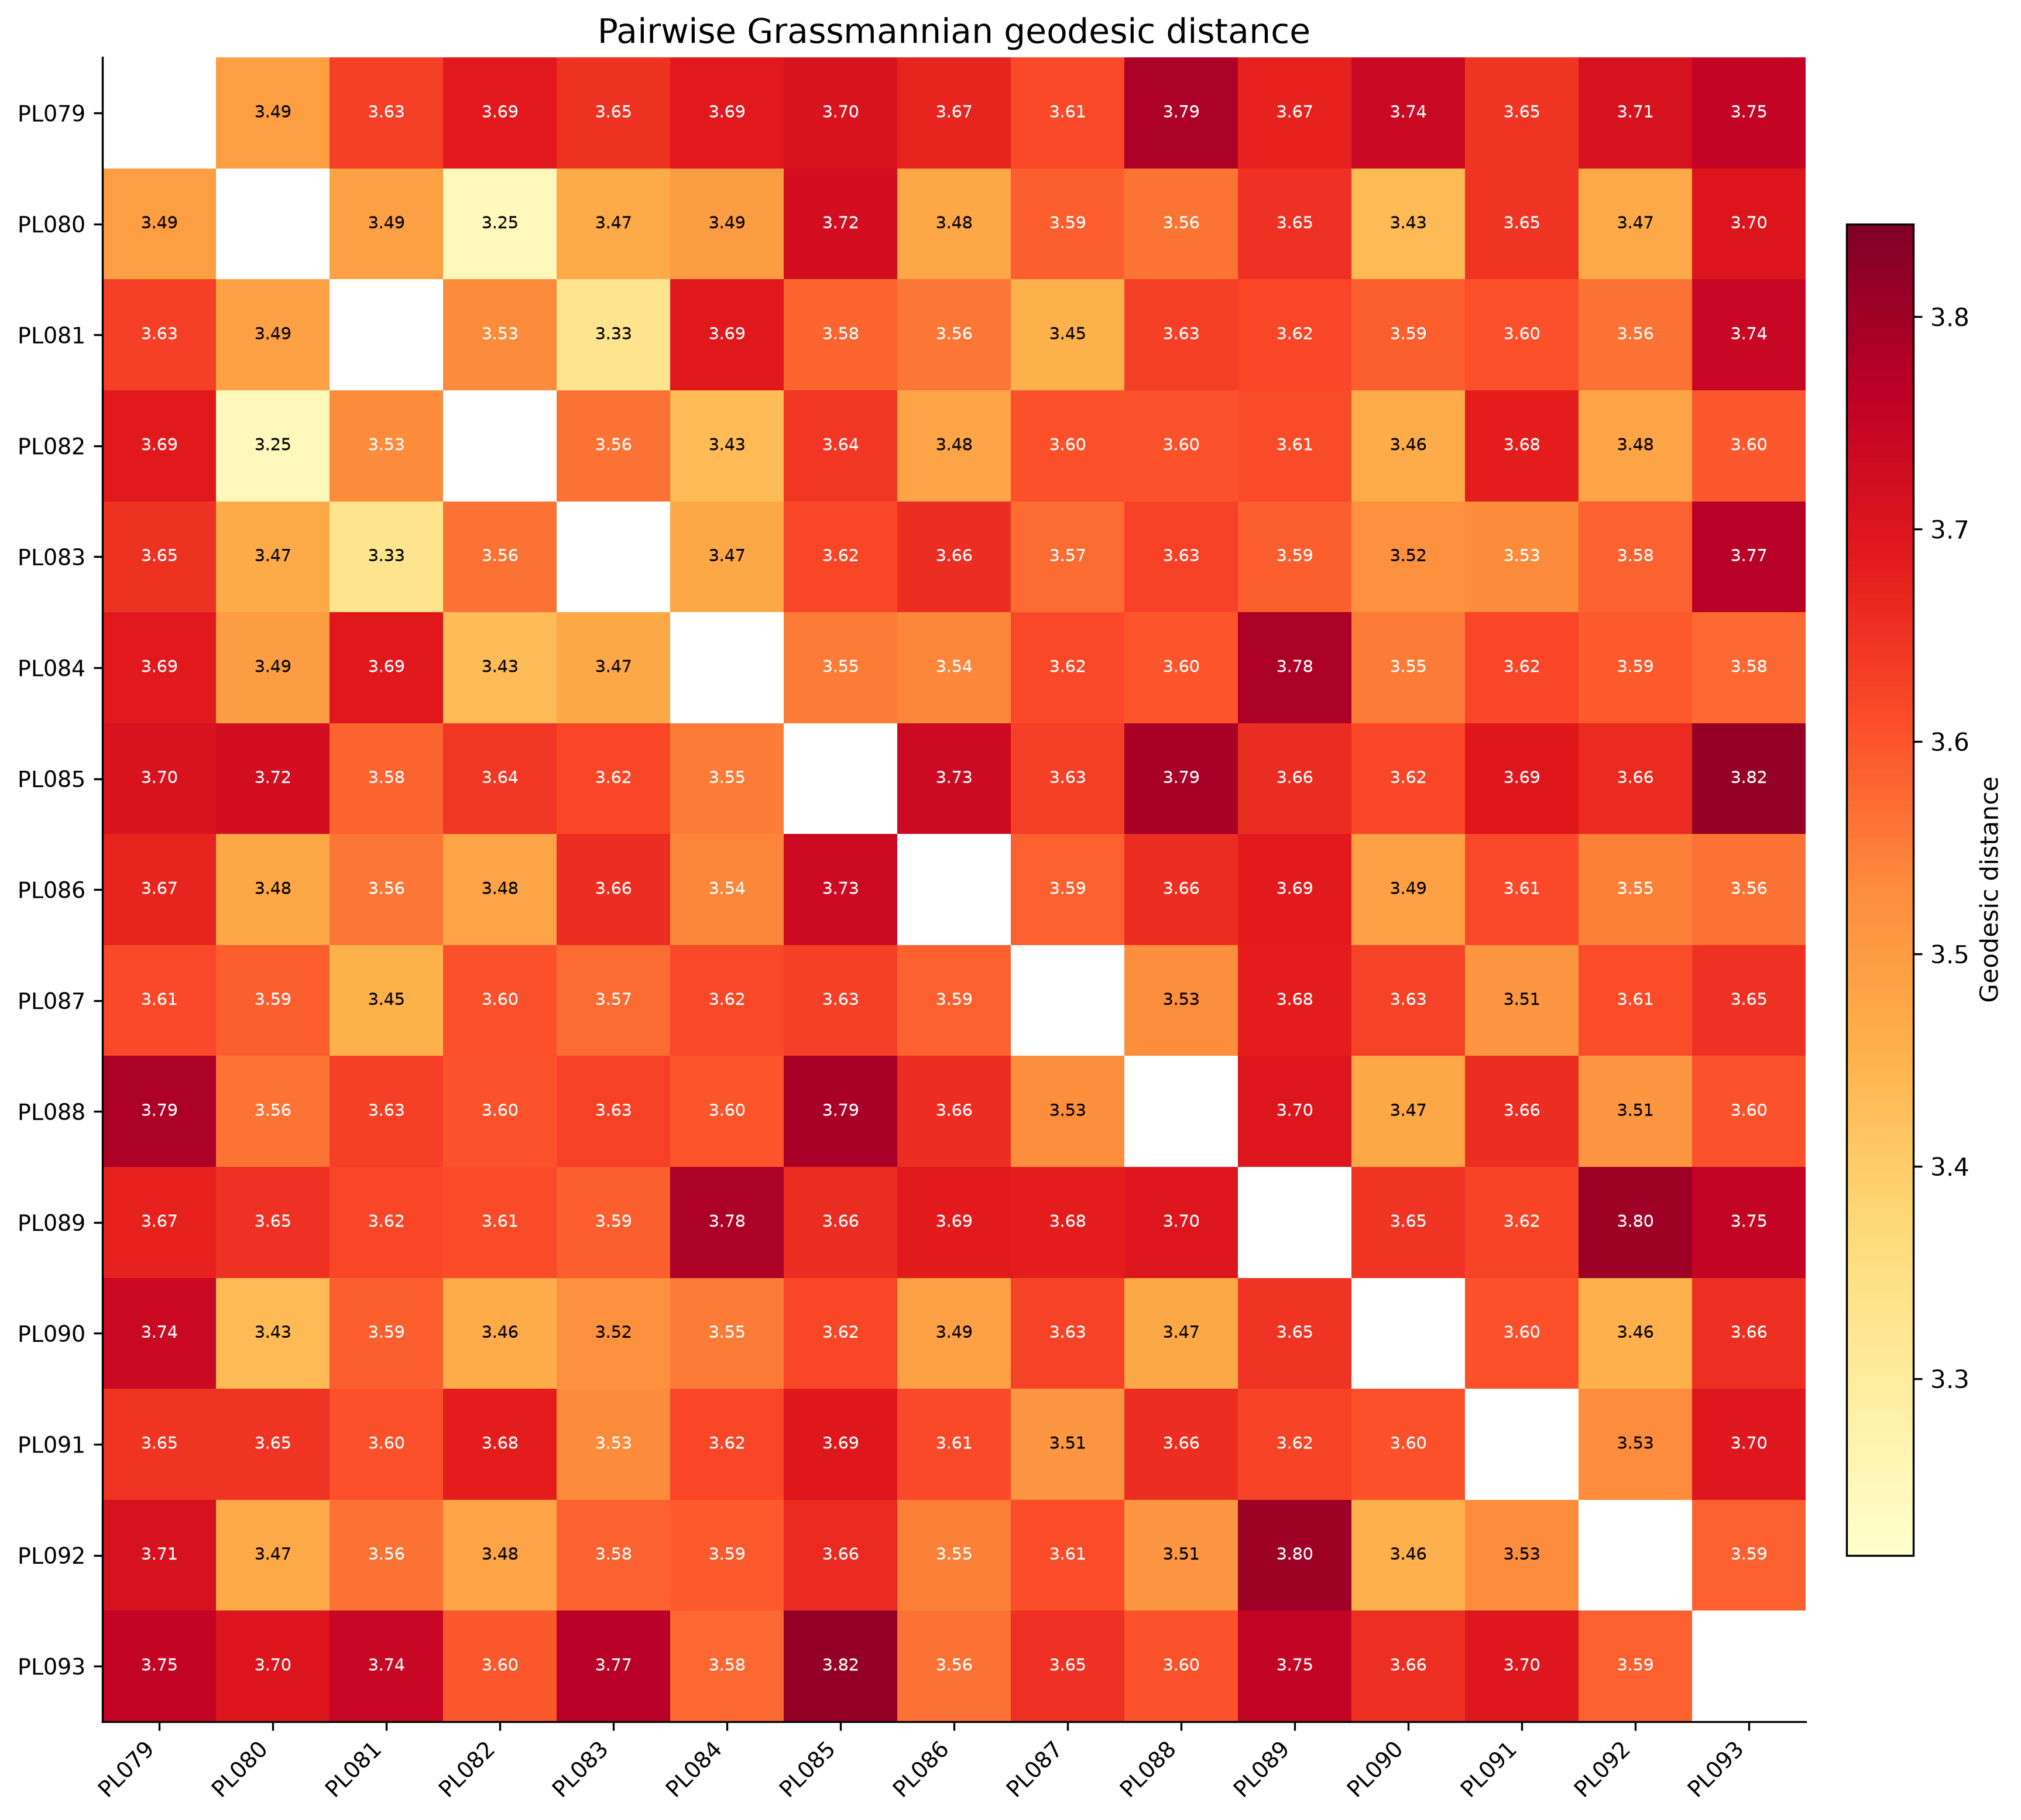
\includegraphics[width=0.9\textwidth]{results/multicohort/figures/F4_distance_heatmap.png}
\caption{Pairwise Grassmannian geodesic distance between plate-specific top-10 PCA subspaces. All 105 off-diagonal entries fall in the range 3.25--3.82. PL080--PL082 is the closest pair; PL085--PL093 the farthest. The narrow range indicates approximately uniform batch-induced subspace shift across all plate pairs.}
\label{fig:heatmap}
\end{figure}

\begin{figure}[t]
\centering
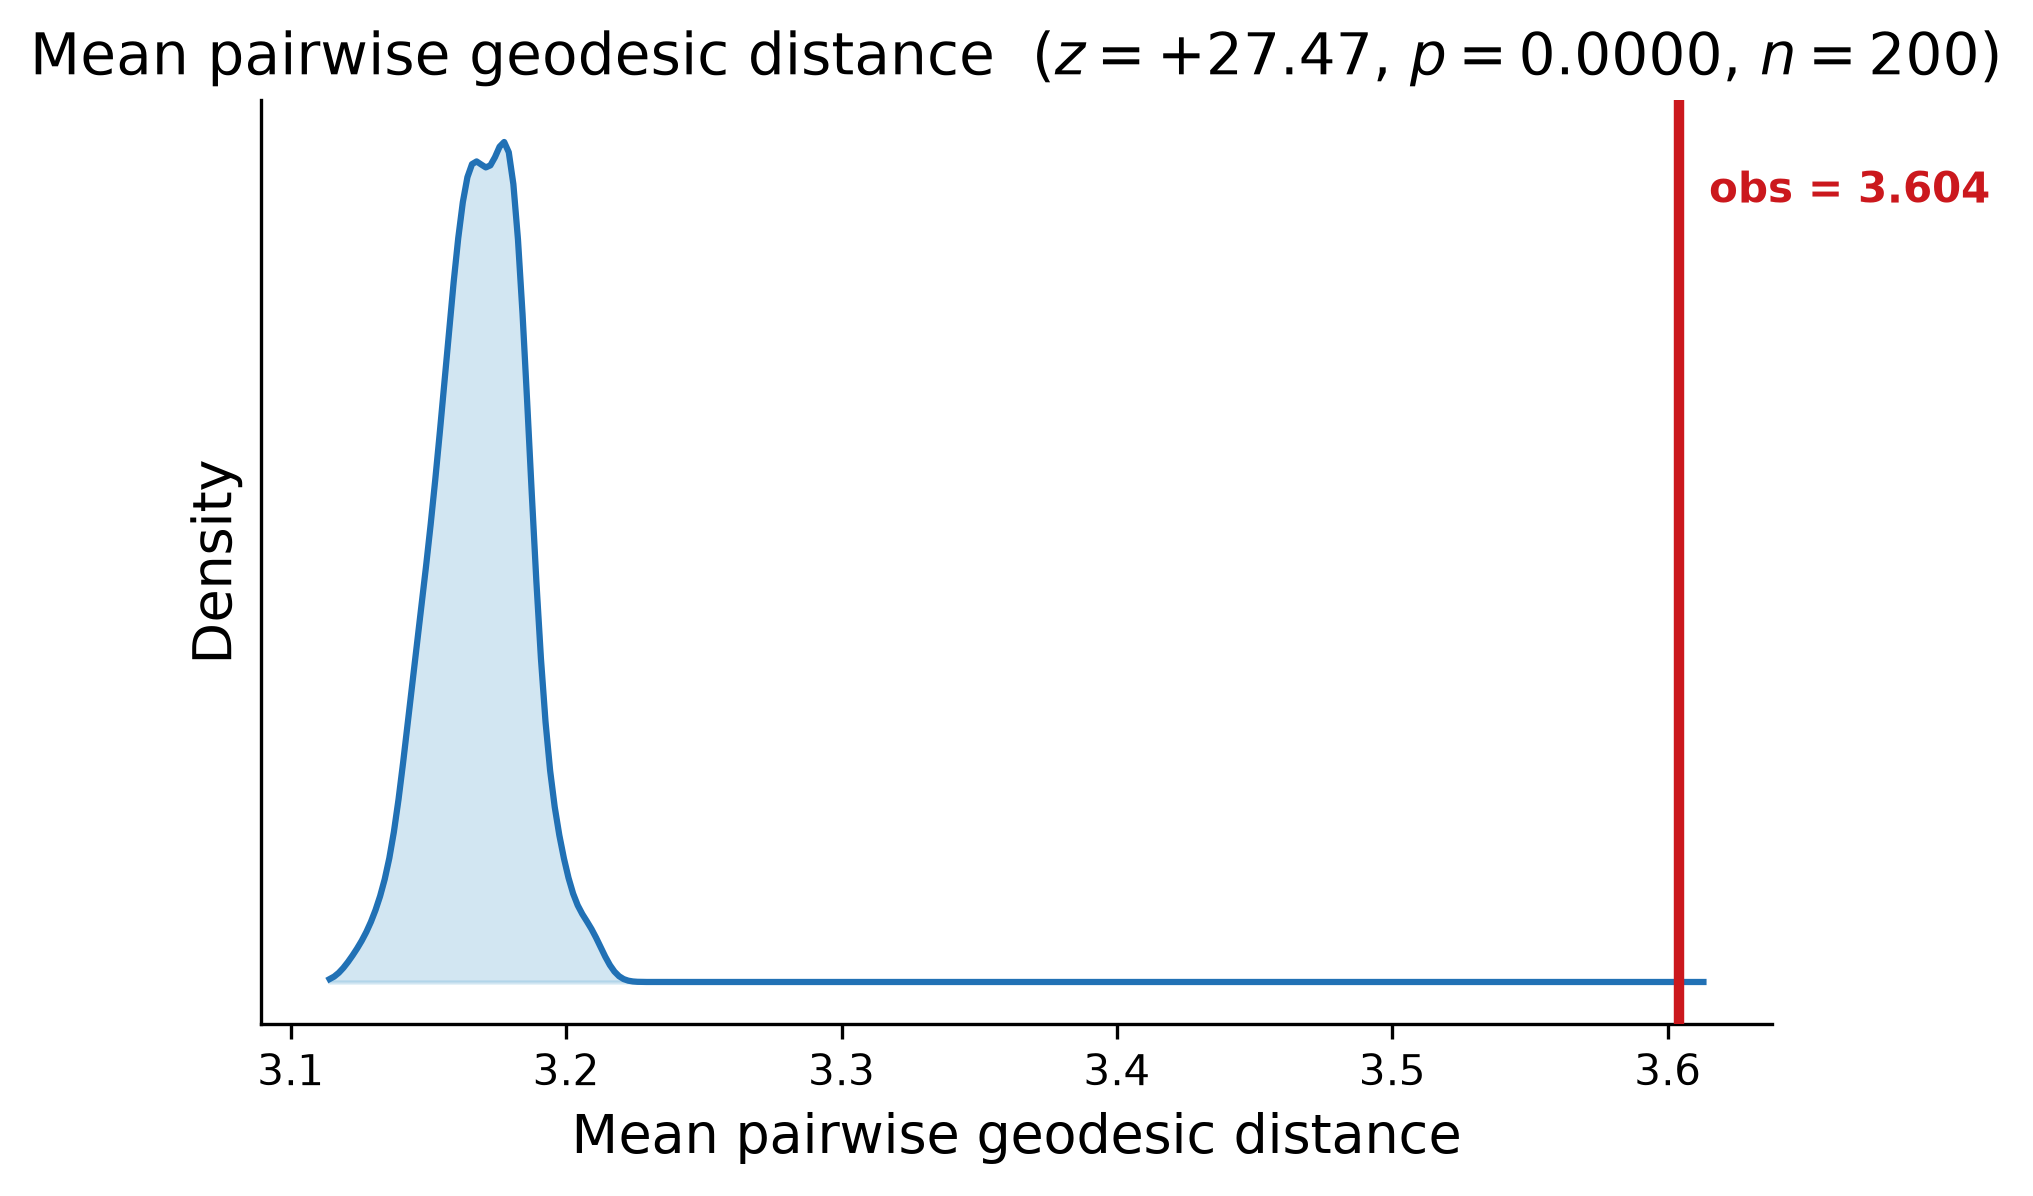
\includegraphics[width=0.7\textwidth]{results/multicohort/figures/F3_null_multicohort.png}
\caption{Mean pairwise geodesic distance (observed $= 3.729$, red line) against the plate-label permutation null (1{,}000 permutations, $z = 31.56$, $p < 0.001$). The null distribution is concentrated around 3.25; the observed value falls entirely outside its support.}
\label{fig:null}
\end{figure}

\paragraph{Principal angle spectra.} The angle spectrum reveals how subspace divergence is distributed across dimensions. For the closest pair (PL080 vs PL082), angles range from 27$^\circ$ to 88$^\circ$; for the farthest (PL085 vs PL093), from 36$^\circ$ to 89$^\circ$ (Figure~\ref{fig:angles}). Even the closest pair has no angles near zero---no principal directions are shared exactly across plates.

\begin{figure}[t]
\centering
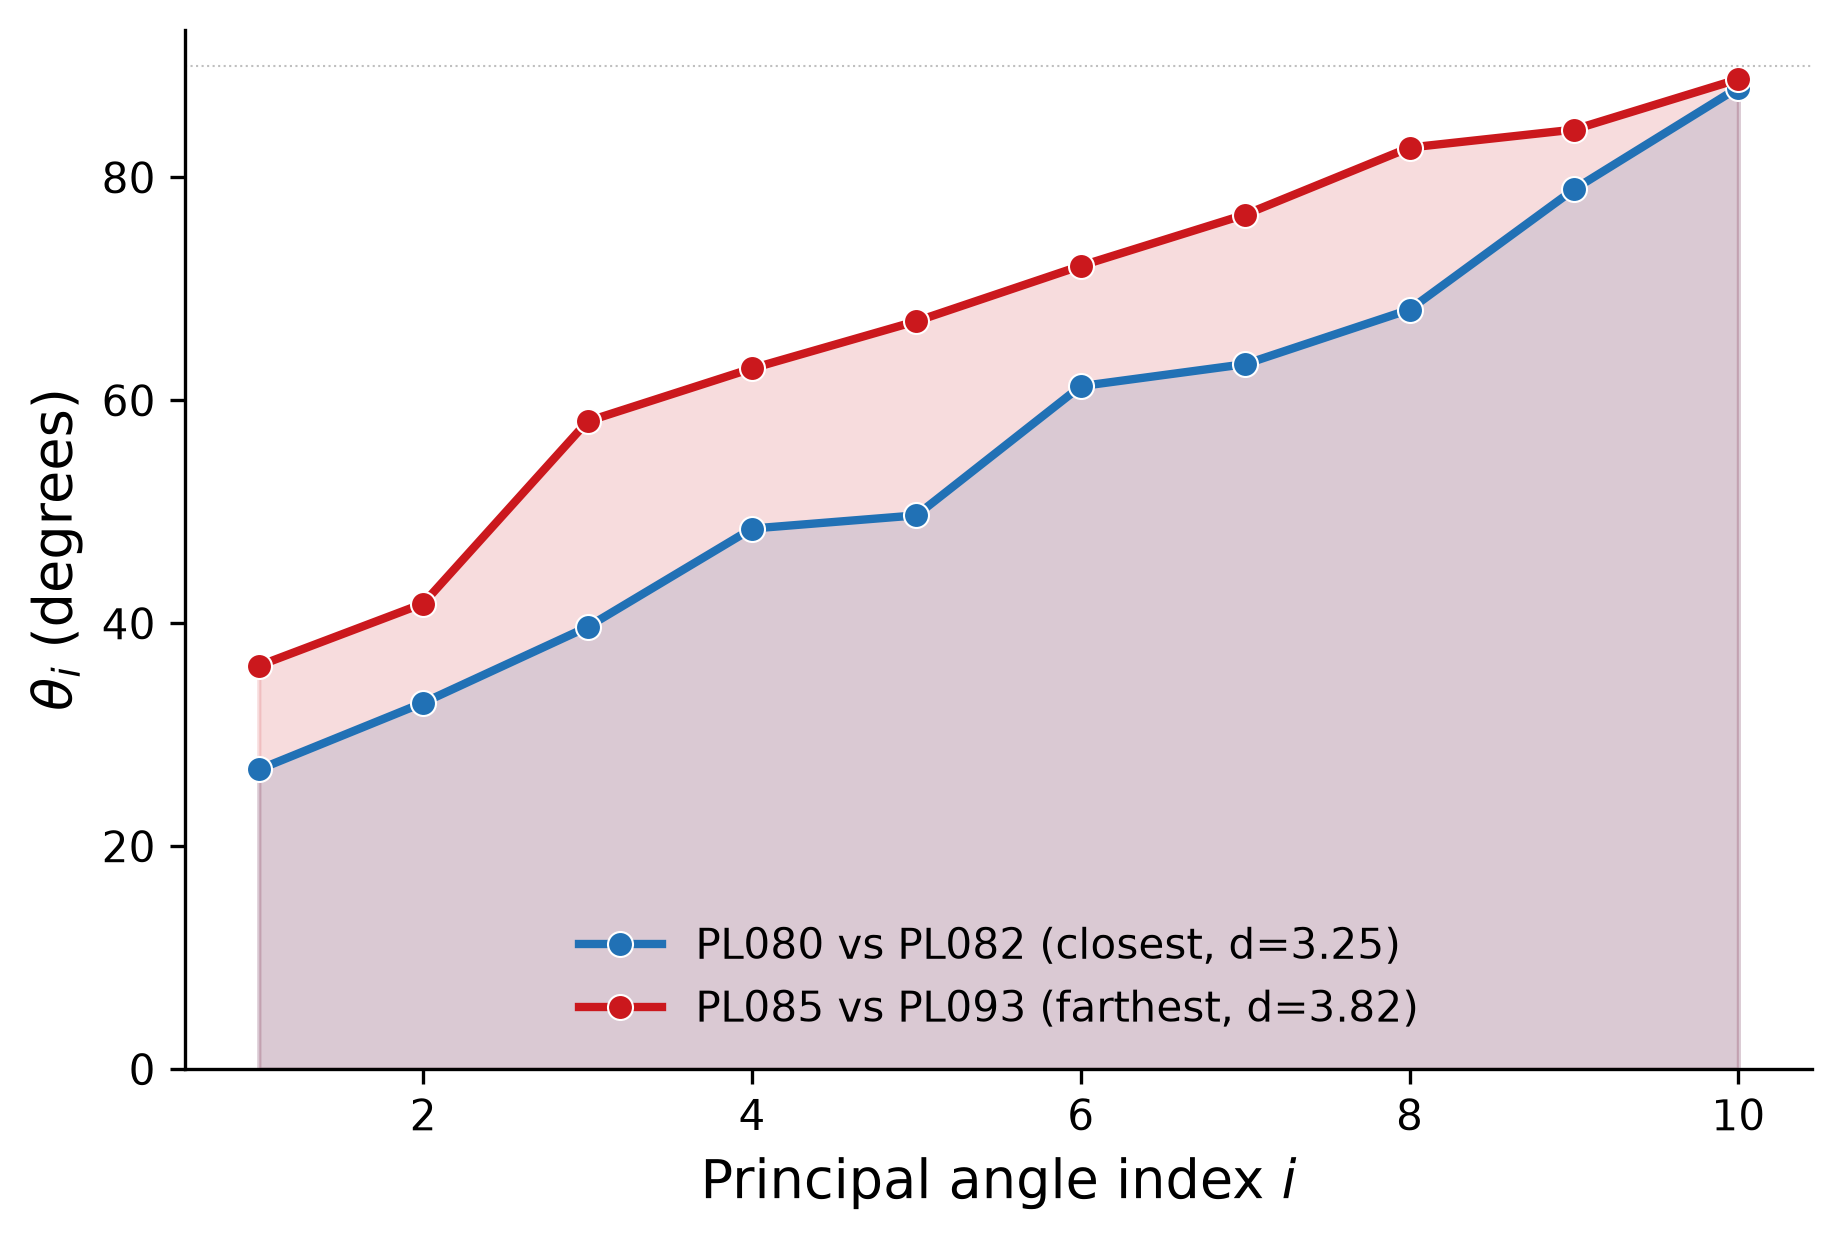
\includegraphics[width=0.7\textwidth]{results/figures/F2c_angle_spectrum_extremes.png}
\caption{Principal angle spectra for the closest (PL080 vs PL082, $d = 3.25$) and farthest (PL085 vs PL093, $d = 3.82$) plate pairs. The farthest pair has uniformly larger angles across all 10 dimensions. Neither pair shares any near-zero angles---all principal directions differ across plates.}
\label{fig:angles}
\end{figure}

\paragraph{Cocycle holonomy.} As a consistency check, we computed parallel transport holonomy around subcycles of 3 and 5 consecutive plates. All Frobenius norms $\|\Phi - I\|_F$ fall in the range $3.7$--$4.5$, confirming that the subspace rotation accumulated around any plate cycle does not close to the identity. Size-5 and size-3 cycles produce comparable holonomy (mean 4.39 vs 4.14), indicating that transport obstruction is dominated by local pairwise misalignment rather than accumulating with cycle length.


\section{Prediction Test: Geodesic Distance vs AUC Gap}
\label{sec:prediction}

The pre-registered hypothesis is that geodesic distance predicts the transportability gap: plates with more divergent subspaces should produce larger drops in classifier performance when one plate's model is evaluated on another.

\paragraph{External validation.} For each of the 105 ordered plate pairs $(i, j)$, we train a classifier on plate $i$ and evaluate on plate $j$, reporting AUC. The ``internal'' AUC is 5-fold cross-validation within the training plate. The AUC gap is defined as internal minus external AUC; positive values indicate the expected direction (external performance worse than internal). We test both logistic regression and random forest classifiers to verify that the result is not classifier-dependent.

\paragraph{Result.} No score predicts the AUC gap at the pre-registered significance level ($\alpha = 0.05$; Table~\ref{tab:baselines}, Figure~\ref{fig:scatter_v2}). For logistic regression, geodesic distance achieves $\rho = 0.040$ ($p = 0.684$). For random forest, the correlation is marginally stronger ($\rho = 0.180$, $p = 0.066$) but still non-significant. Three na\"{i}ve baselines---centroid distance, domain-classifier AUC, and variance ratio---perform comparably, with the best (variance ratio vs logistic regression gap) reaching $\rho = 0.188$ ($p = 0.054$).

\begin{table}[t]
\centering
\caption{Spearman $\rho$ between each distributional score and the AUC gap, for logistic regression and random forest classifiers. No score reaches the pre-registered $\alpha = 0.05$ threshold. The Fisher-Rao confound fraction is constant at zero across all 105 pairs (the label-conditioned shift exceeds the raw centroid shift for every pair) and is omitted. Domain-classifier AUC saturates near 1.0 for all pairs (mean 1.000, range [0.986, 1.000]), confirming that plates are always distinguishable at the sample level.}
\label{tab:baselines}
\begin{tabular}{lcccc}
\toprule
 & \multicolumn{2}{c}{Logistic Regression} & \multicolumn{2}{c}{Random Forest} \\
\cmidrule(lr){2-3} \cmidrule(lr){4-5}
Score & $\rho$ & $p$ & $\rho$ & $p$ \\
\midrule
Grassmannian geodesic    & $+$0.040 & 0.684 & $+$0.180 & 0.066 \\
Centroid distance        & $+$0.157 & 0.110 & $+$0.009 & 0.928 \\
Domain-classifier AUC    & $-$0.092 & 0.350 & $+$0.047 & 0.634 \\
Variance ratio           & $+$0.188 & 0.054 & $-$0.050 & 0.612 \\
\bottomrule
\end{tabular}
\end{table}

\begin{figure}[t]
\centering
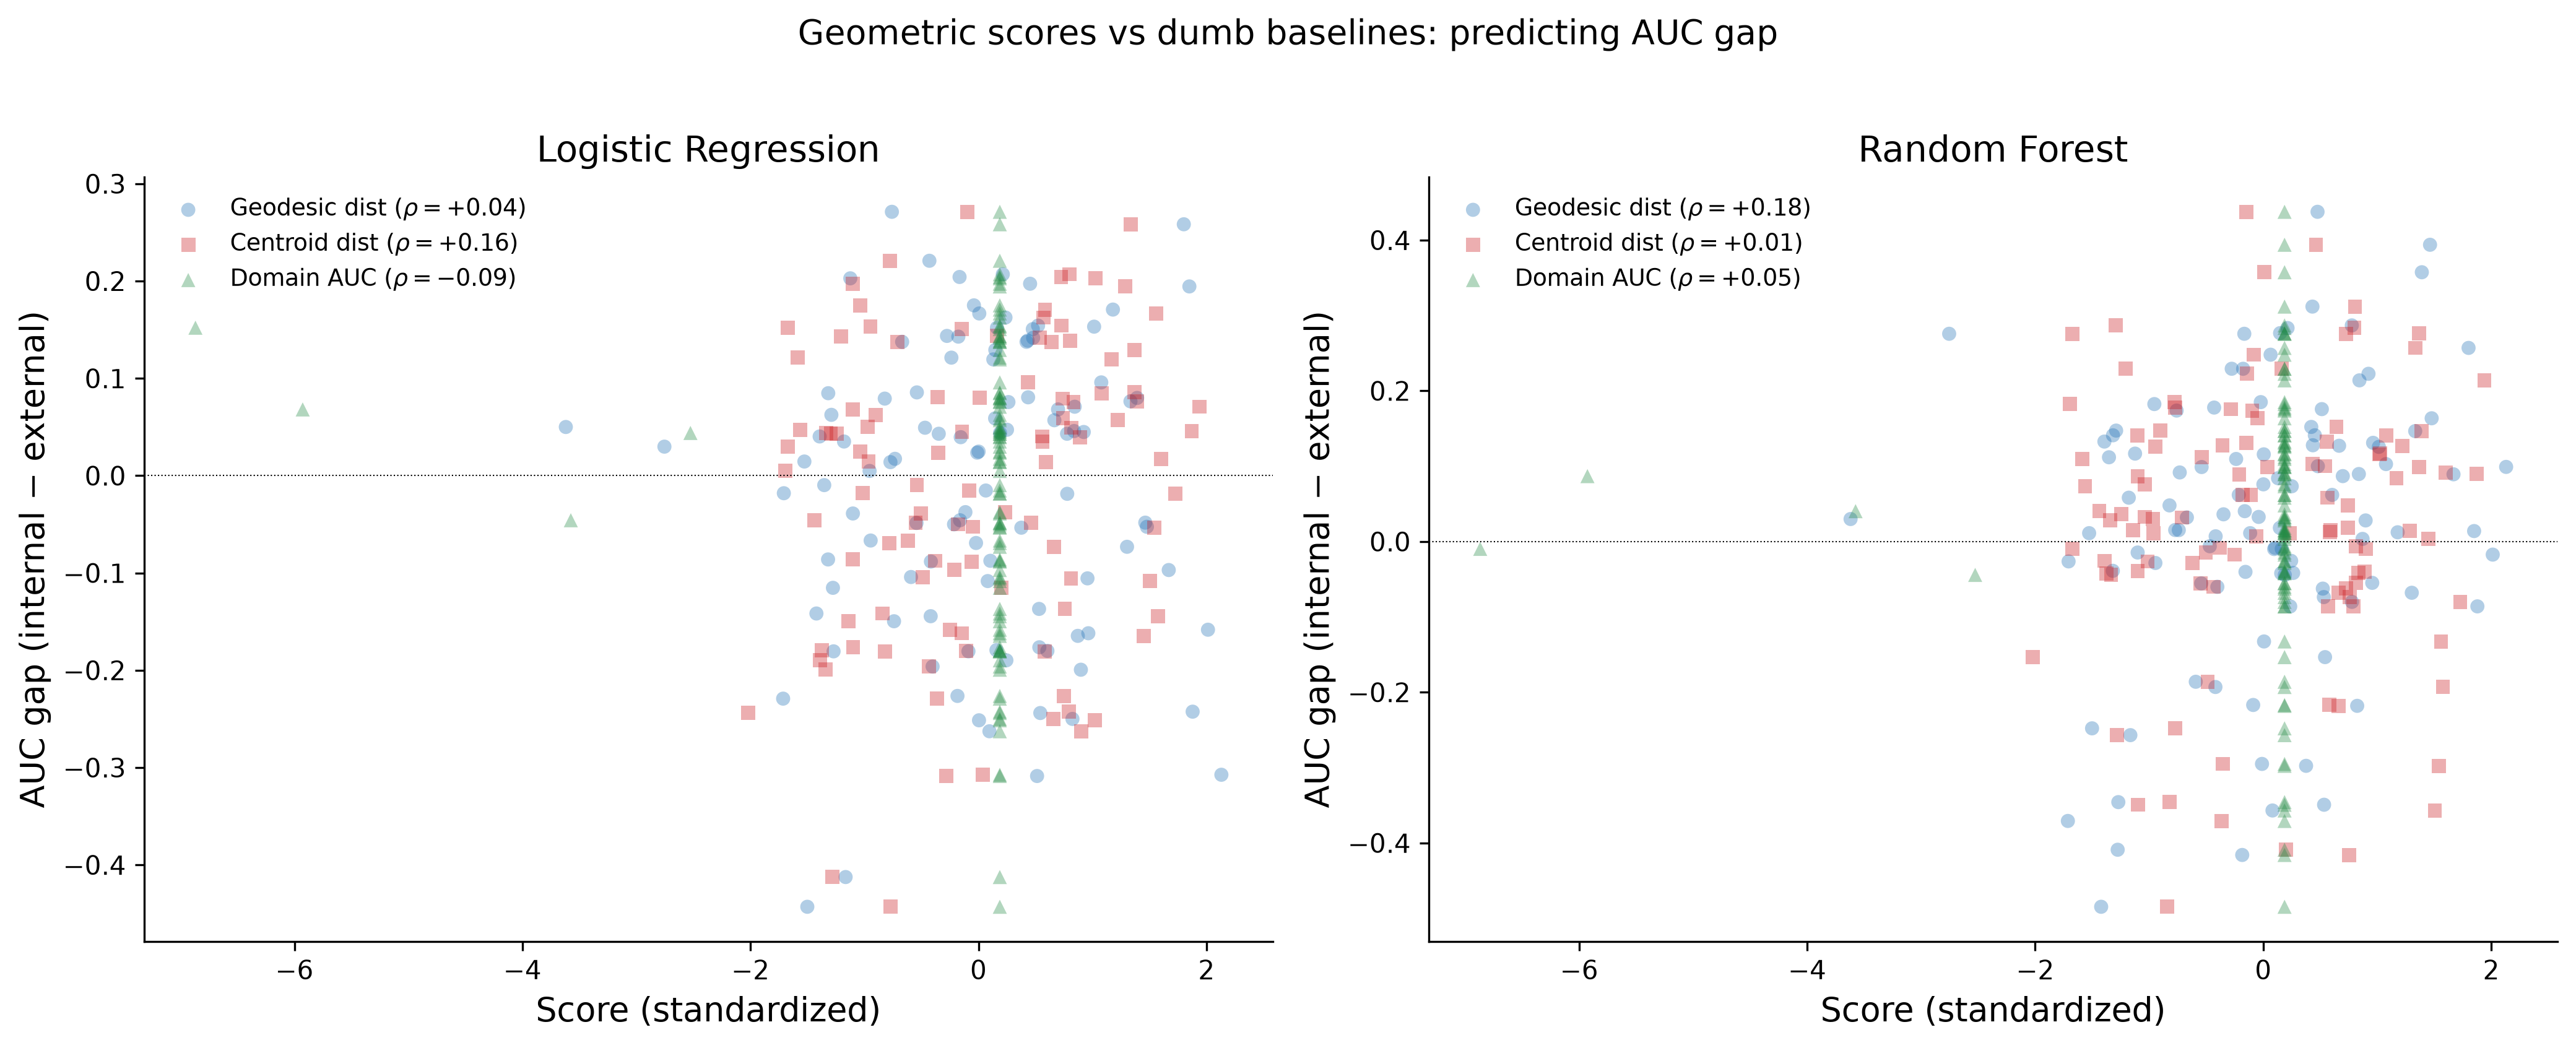
\includegraphics[width=\textwidth]{v2/results/figures/F1_v2_scatter_with_baselines.png}
\caption{Geodesic distance, centroid distance, and domain-classifier AUC (standardized) vs pairwise AUC gap, for logistic regression (left) and random forest (right). All correlations are weak. The geodesic score shows a marginal positive trend for random forest ($\rho = 0.180$, $p = 0.066$), while centroid distance shows a comparable trend for logistic regression ($\rho = 0.157$, $p = 0.110$). Neither reaches significance.}
\label{fig:scatter_v2}
\end{figure}

\paragraph{Diagnosis.} Two factors explain the null result. First, per-plate sample sizes ($\sim$72 samples, $\sim$12 positives) produce AUC estimates with standard errors of $\sim$0.10, comparable to the total range of AUC gaps observed ($-0.44$ to $+0.44$). Any geometric signal is undetectable against this measurement noise. Second, the geodesic distances themselves are compressed: a coefficient of variation of 3.5\% means all plates are roughly equidistant, leaving little dynamic range for a correlation to emerge. A dataset with cohorts spanning a wider range of batch severity---different instruments, laboratories, or time periods---would provide a stronger test.

\paragraph{Baseline saturation.} The domain-classifier AUC saturates near 1.0 for all 105 pairs (range [0.986, 1.000]): a logistic regression can always distinguish which plate a sample came from. This confirms that plates are distributionally distinct at the sample level, consistent with the permutation-null result, but provides no usable variance for predicting the AUC gap. The Fisher-Rao confound score---which decomposes cross-cohort centroid shift into batch and label-conditioned components---is constant at zero across all pairs, indicating that the label-specific centroids (cancer vs healthy) shift by more than the overall centroids. In this dataset, label geometry and batch geometry are entangled in a way that the Fisher-Rao decomposition cannot resolve.

\paragraph{AUC gap structure.} The pairwise AUC gap matrix (Figure~\ref{fig:aucgap}) shows asymmetric structure: training on PL079 and testing on PL080 yields $+0.26$ gap, while the reverse yields $-0.26$. Rows with consistently positive gaps (PL079, PL084) indicate plates whose classifiers generalize poorly; rows with negative gaps (PL085, PL086) indicate plates whose classifiers transfer well. This asymmetry is invisible to the symmetric geodesic distance, and may reflect label distribution or feature quality differences across plates.

\begin{figure}[t]
\centering
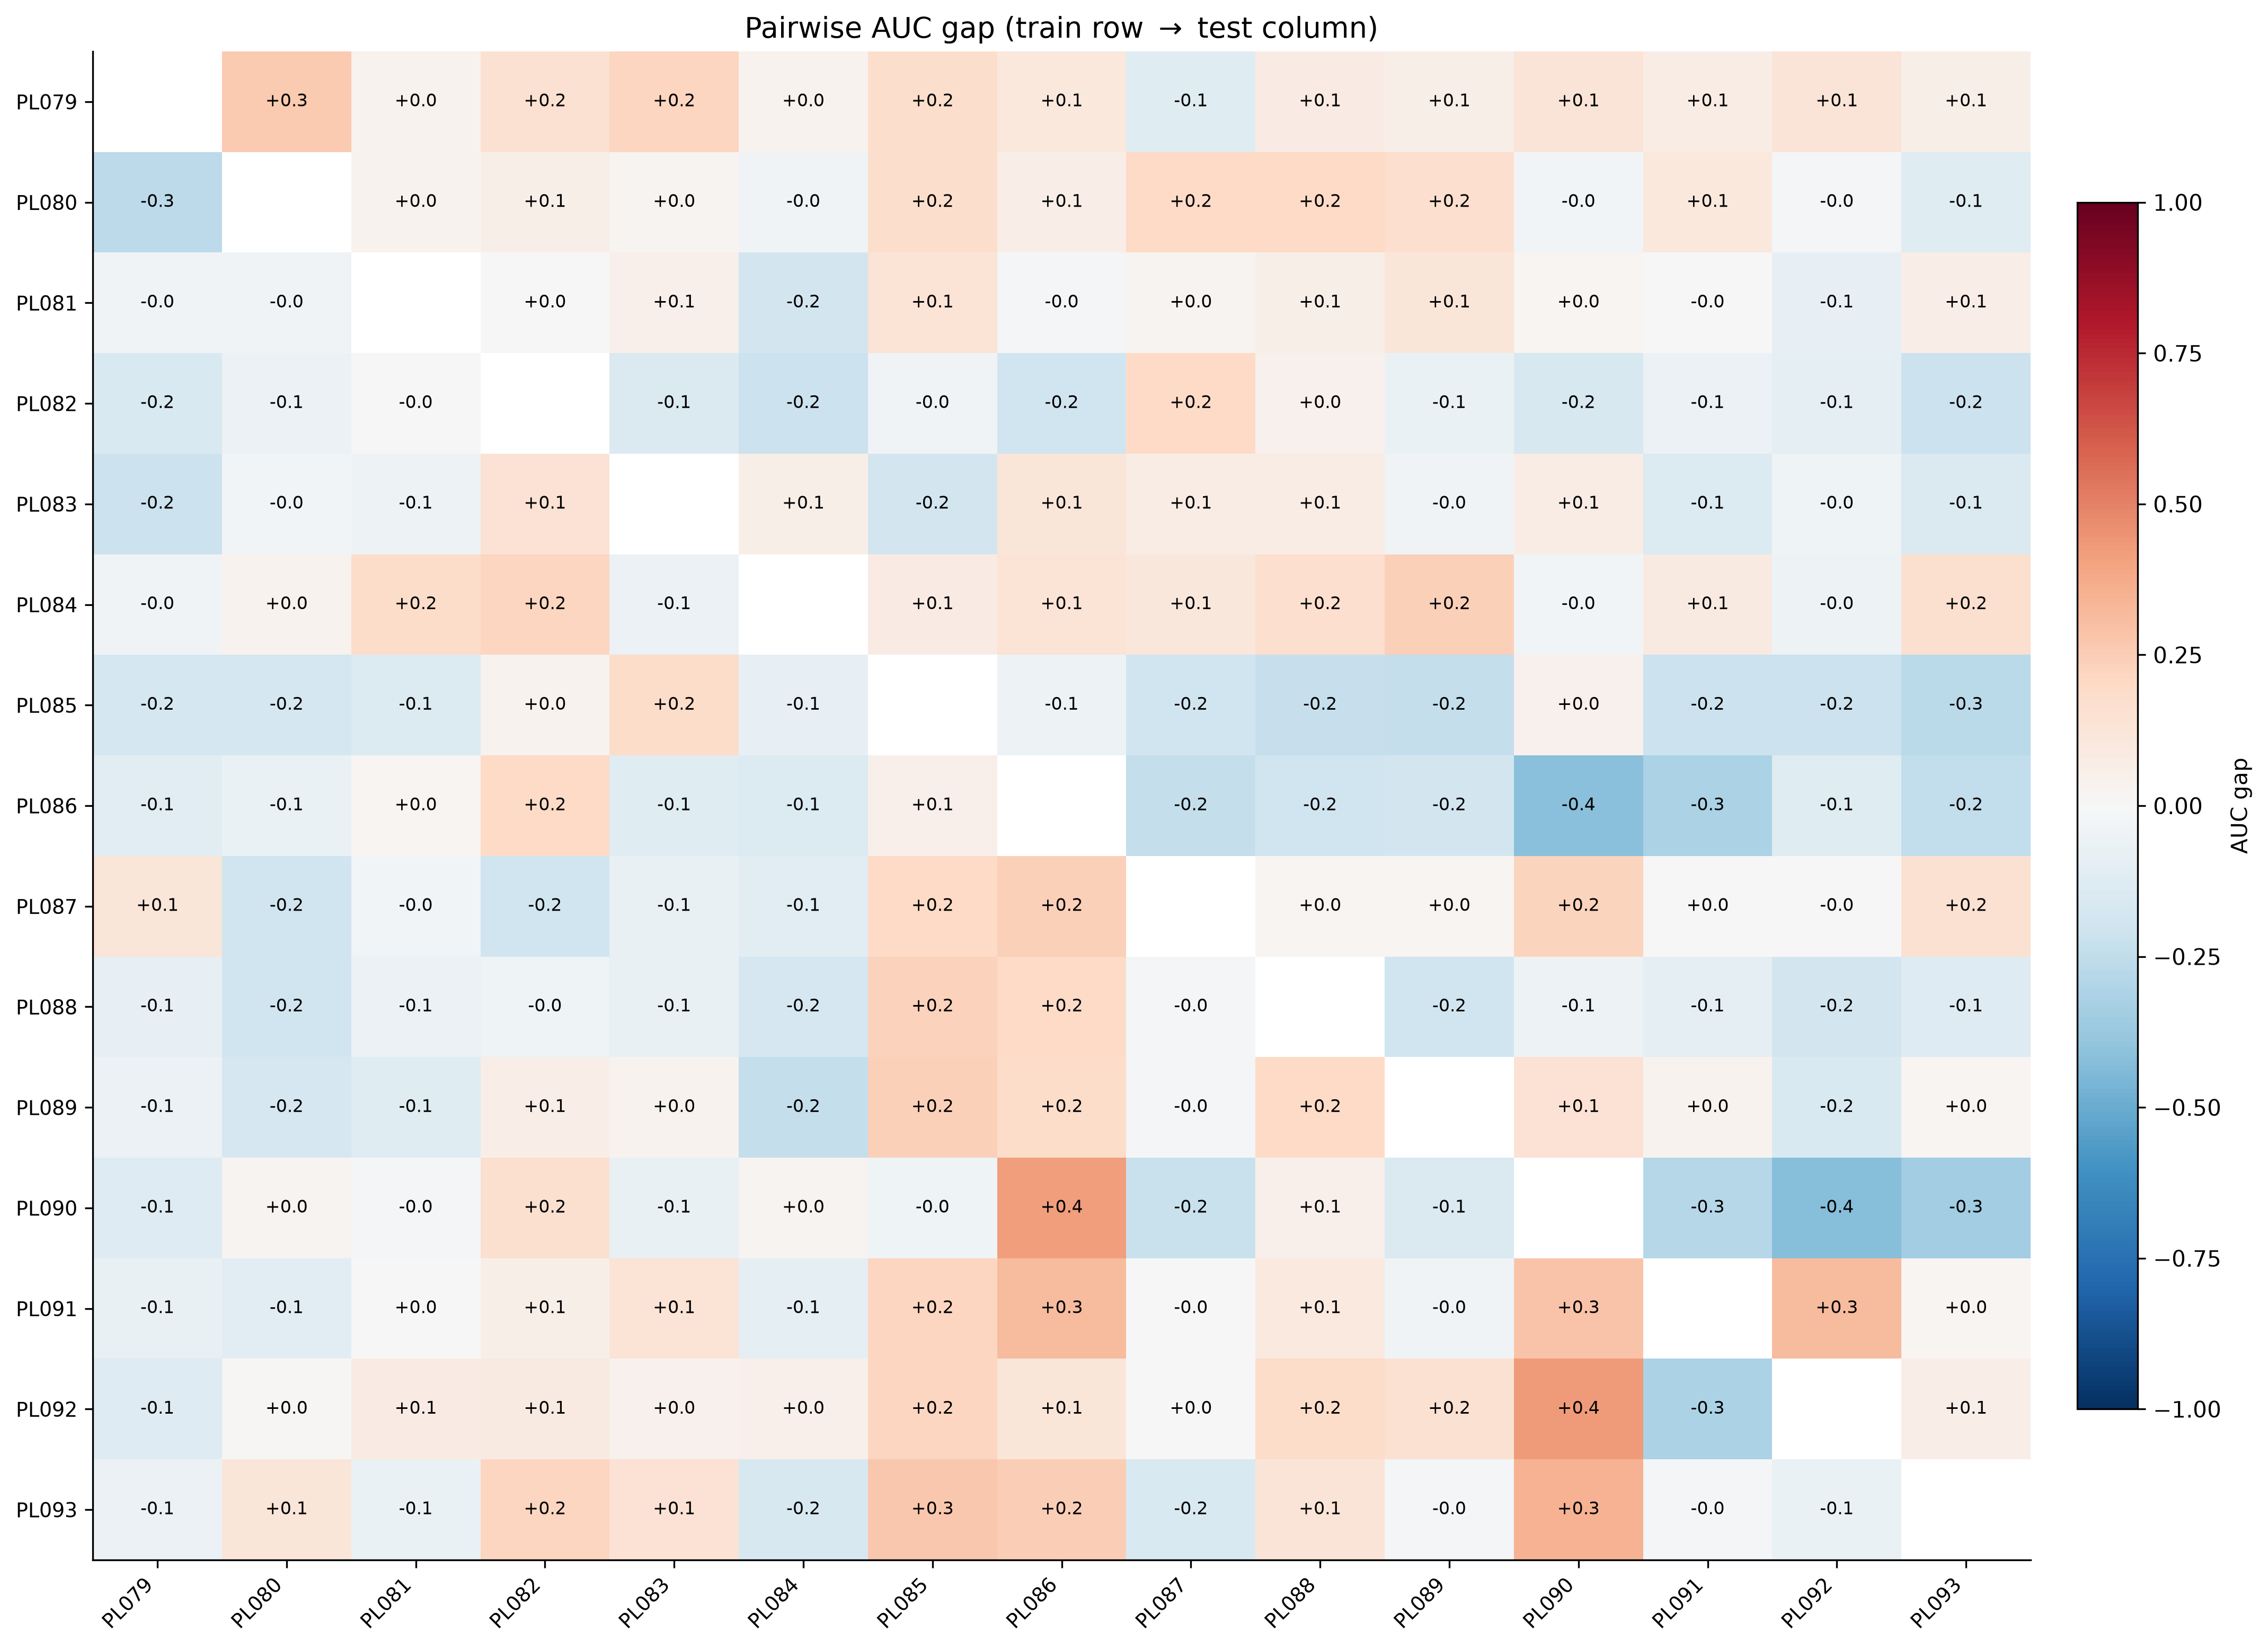
\includegraphics[width=0.9\textwidth]{results/multicohort/figures/F5_auc_gap_heatmap.png}
\caption{Pairwise AUC gap (train row, test column). Positive values (red) indicate worse external than internal performance; negative (blue) indicate better. PL079 and PL084 are consistently poor senders; PL085 and PL086 are consistently poor receivers. Geodesic distance is symmetric and cannot capture this directional structure.}
\label{fig:aucgap}
\end{figure}


\section{Discussion}
\label{sec:discussion}

\paragraph{What the geometry detects.} Grassmannian geodesic distance detects batch-induced subspace divergence in this metabolomics dataset. The $z = 31.56$ separation from the permutation null is clear: plates occupy distinct regions of the Grassmannian, and this structure is not an artifact of sample-level variance.

\paragraph{What the geometry does not predict.} Batch-structure detection is necessary but insufficient for predicting transportability failure. The prediction test fails ($\rho = 0.040$, $p = 0.684$) because the per-plate samples are too small for stable AUC estimation. The geodesic distances and AUC gaps operate at different signal-to-noise ratios: geometry aggregates across all 1{,}022 features and is estimated from the full plate covariance, while AUC depends on $\sim$12 positive labels per plate.

\paragraph{Baselines confirm the null.} All three na\"{i}ve baselines (centroid distance, domain-classifier AUC, variance ratio) also fail to predict the AUC gap ($|\rho| \leq 0.188$, all $p > 0.05$). The geodesic score does not outperform these simpler measures. This suggests that the limiting factor is AUC estimation noise, not the choice of distributional score: when the outcome variable has standard errors of $\sim$0.10 on a signal range of $\sim$0.5, no predictor can achieve a meaningful correlation at $n = 105$.

\paragraph{Asymmetry.} The AUC gap is asymmetric (training on plate $A$ and testing on $B$ differs from the reverse), while geodesic distance is symmetric. A directional geometric measure---such as the projection of the between-cohort shift onto the classification-relevant subspace---could capture this asymmetry.

\paragraph{Limitations.}

\begin{itemize}
\item All results are retrospective on one public dataset (MTBLS7260). Generalization to other omics platforms, diseases, and sample sizes is untested.
\item Per-plate sample sizes ($\sim$72, $\sim$12 positives) are too small for the prediction test. A dataset with fewer, larger cohorts would be more informative.
\item Geodesic distances are compressed (CV 3.5\%), limiting the dynamic range for correlation. Datasets with cohorts from different instruments or laboratories would provide wider separation.
\item We use PCA subspaces as the representation. Nonlinear embeddings might produce different subspace structure.
\item Both classifiers (logistic regression and random forest) are diagnostic tools for measuring the AUC gap, not optimized clinical models.
\end{itemize}

\paragraph{Conclusion.} Grassmannian geodesic distance provides a well-defined geometric test for batch structure in metabolomics: plates are detectably distinct ($z = 31.56$) and the closest and farthest plate pairs are identifiable from their principal angle spectra. Translating this geometric detection into quantitative prediction of classifier degradation remains open. The limiting factor is not the geometric measure---na\"{i}ve baselines also fail---but the AUC estimation noise inherent in small per-cohort sample sizes.

\bibliography{references}
\bibliographystyle{tmlr}

\end{document}
